\section{Transformadores}
\label{sec:unidad-transformadores}
\subsection{Transformadores Ideales}
\subsubsection{Principio de funcionamiento}
Para el análisis se toma que el transformador está alimentado por el lado de alta (el de más espiras) y trabaja como un reductor. Es decir que:

\begin{enumerate}
	\item El primario trabaja como un recepto respecto a la fuente (recibe corriente).
	\item El secundario se comporta como un generador respecto a la carga conectada a sus bordes (entrega coriente).
\end{enumerate}

Para un transformador ideal no existen pérdidas por histéresis y corrientes parásitas, y no existen flujos de dispersión (todo el flujo magnético enlaza al primario y secundario).

\subsubsection{Transformador ideal sin carga}

\begin{figure}[h]
	\vspace{-1cm}
	\centering
	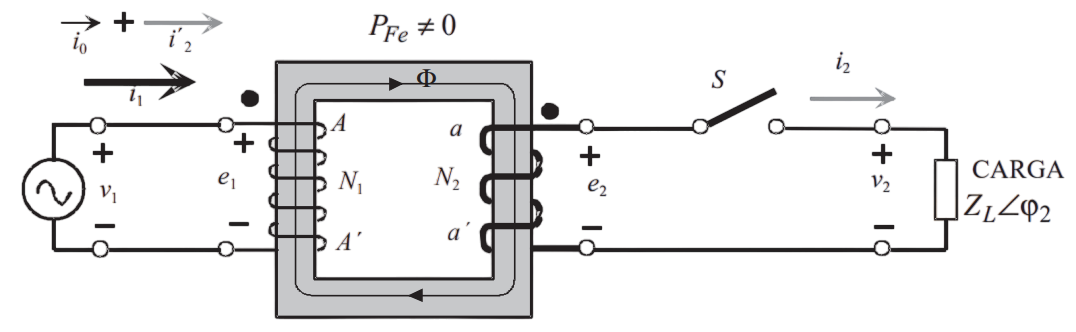
\includegraphics[width=0.80\linewidth]{trafo-ideal}
	\caption{Esquema de un transformador ideal}
	\label{fig:transformador-ideal}
\end{figure} 
 
 Realmente $e_{1}$ representa una f.c.e.m porque se opone a $v_{1}$ y limita la corriente de primario. La polaridad $e_{2}$ tiene en cuenta que, al cerrar el circuito,\footnote{Porque si está abierto, sólo hay tensión y no corriente} la corriente $i_{2}$ debe generar un flujo que se oponga el flujo primario que la originó. Es decir que, \textsl{la f.m.m del secundario actúa en contra de la f.m.m primaria produciendo un efecto desmagnetizante sobre ésta.}\\
 
 
 Aplicando la 2° Ley de Kirchhoff al transformador ideal tenemos que:
 
\begin{equation}
	v_1 = e_1 = N_1 \dfrac{d\Phi}{dt} \hspace{.5cm};\hspace{.5cm} e_2 = v_2 = N_2 \dfrac{d\Phi}{dt}
	\label{eq:voltaje}
\end{equation}

Si se parte de un flujo \textbf{senoidal} de la forma:
\begin{equation}
	\Phi = \Phi_m \sin{\omega t} = \Phi_m \cos\left(\omega t - 90\deg\right)
\end{equation}

Haciendo la derivada del flujo y reemplazando en \ref{eq:voltaje} tenemos:
\begin{equation*}
	\begin{split}
		v_1 = e_1 = N_1 \omega \Phi_m \cos\left(\omega t\right) \\
		e_2 = v_2 = N_2 \omega \Phi_m \cos\left(\omega t\right)
	\end{split}
\end{equation*}

Comparando el flujo expresado en coseno y los voltajes podemos ver que en estos últimos van 90° adelantados respecto al flujo, se podría decir entonces que la corriente va en fase con el flujo magnético. 

Si calculamos sus \textbf{valores eficaces}:

\begin{equation}
	\begin{split}
		V_1 = E_1 = \dfrac{N_1 \omega \phi_m}{\sqrt{2}} = 4,44 f N_1 \Phi_m \\
		V_2 = E_2 = \dfrac{N_2 \omega \phi_m}{\sqrt{2}} = 4,44 f N_2 \Phi_m
	\end{split}
\end{equation}

Dividiendo entre sí las ecuaciones y simplificando resulta:

\begin{equation}
	\dfrac{V_1}{V_2} = \dfrac{E_1}{E_2} = \dfrac{N_1}{N_2} = m
\end{equation} 

donde el factor \textit{m} se denomina \textbf{relación de transformación}.\\

Si el transformador está en \textbf{vacío} o \textbf{sin carga}, las pérdidas en el hierro $P_{Fe}$ en el núcleo del transformador será:
\begin{equation}
	P_{Fe} = V_{1} I_{0} \cos \left(\phi_{0}\right)
\end{equation}

donde $V_{1}$ y $I_{0}$ representan los valores eficaces de la tensión y la corriente.\\

La corriente de vacío $I_{0}$ tiene dos componentes: una activa $I_{Fe}$ y una reactiva $I_{\mu}$.

 \begin{figure}[!htbp]
	\centering
	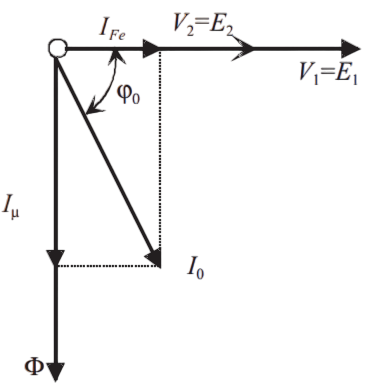
\includegraphics[width=0.3\linewidth]{vacio-fasores}
	\caption{Diagrama fasorial de tensiones y corrientes en vacío.}
	\label{diag:vacio}
\end{figure} 

\subsubsection{Transformador ideal con carga}

En la figura \ref{fig:transformador-ideal} si cerramos el interruptor S, el transformador funciona \textbf{en carga} y aparece una corriente $i_{2}$ que circula por el secundario.

\begin{equation*}
	\fasor{I}_2 = \dfrac{\fasor{e}_2}{\fasor{Z}_L} = \dfrac{E_2 \angle 0}{Z_L \angle \phi_2} = \dfrac{E_2}{Z_L} \angle -\phi_2
\end{equation*}

La corriente $\fasor{i}_2$ se retrasa $\phi_{2}$ de la f.m.m $\fasor{e}_2$. \\


La corriente $i_{2}$ en el secundario produce una f.m.m. desmagnetizante $N_{2}i_{2}$ que se opone a la f.m.m primaria $N_{1}i_{0}$. Para que el flujo no se vea reducido por este efecto, en el primario se genera una corriente adicional primaria $i'_{2}$ con una f.m.m equivalente:

\begin{equation*}
	N_1 i_2'=N_2 i_2
\end{equation*}

de donde se deduce el valor de la corriente $i'_{2}$ adicional primaria:

\begin{equation}
	i_2' = \dfrac{N_2}{N_1} i_2 = \dfrac{i_2}{m}
\end{equation}

La corriente total necesaria en el primario $i_{1}$ será igual a:

\begin{equation*}
	i_1 = i_0 + i_2' = i_0 + \dfrac{i_2}{m}
\end{equation*}

Y en forma fasorial: 

\begin{equation}
	\fasor{i}_1 = \fasor{i}_0 + \fasor{i}_2' = \fasor{i}_0 + \dfrac{\fasor{i}_2}{m}
	\label{eq:corriente1}
\end{equation}

La ecuación \ref{eq:corriente1} nos indica que la corriente primaria $\fasor{i}_{1}$ tiene dos componentes:

\begin{itemize}
	\item \textbf{Una corriente de excitación o de vacío} $\fasor{i}_0$ que produce el flujo en el núcleo magnético y vence las pérdidas en el hierro a través de sus componentes $\fasor{i}_{\mu}$ y $\fasor{i}_{Fe}$;
	\item Y \textbf{una componente de carga} $\fasor{i}_2'$ que equilibra o contrarresta la acción desmagnetizante de la f.m.m secundaria para que el flujo en el núcleo permanezca constante e independiente de la carga. Esta se denomina \textbf{corriente secundaria reducida}.
\end{itemize}

A plena carga la corriente $\fasor{i}_2'$ es 20 veces por lo menos mayor que $\fasor{i}_0$ por lo que puede despreciarse y la ecuación queda:

\begin{center}
	$\fasor{i}_1 \approx \fasor{i}_2' = \dfrac{\fasor{i}_2}{m}$
\end{center}

\subsection{Funcionamiento de un transformador real}

En el análisis de un trafo real se tiene en cuenta la resistencias $R_{1}$ y $R_{2}$ de los arrollamientos y los flujos de dispersión $\Phi_{d1}$ y $\Phi_{d2}$ que se cierran en el aire.

Si consideramos los flujos de dispersión desaparece la idea del flujo común único que existía en el transformador ideal. Si tomamos que $\Phi_{1}$ y $\Phi_{2}$ son los flujos totales que atraviesan los devanados primario y secundario y $\Phi$ es el flujo común a ambos se cumplirá:

\begin{equation*}
	\begin{split}
		\Phi_1 = \Phi + \Phi_{d1} \\
		\Phi_2 = \Phi + \Phi_{d2}
	\end{split}
\end{equation*}

Para representar estas pérdidas agregamos las resistencias $R_{1}$ y $R_{2}$ y dos bobinas adicionales con núcleo de aire que representan los flujos de dispersión $\Phi_{d1}$ y $\Phi_{d2}$ donde se han indicado con $L_{d1}$ y $L_{d2}$ a los coeficientes de autoinducción, cuyos valores serán:

\begin{equation*}
	\begin{split}
		L_{d1} = N_1 \dfrac{d\Phi_{d1}}{di_1} \\
		L_{d2} = N_2 \dfrac{d\Phi_{d2}}{di_2}
	\end{split}
\end{equation*}

y que dan lugar a las reactancias de dispersión $X_{1}$ y $X_{2}$ de ambos devanados:
\begin{equation*}
	\begin{split}
		X_1 = L_{d1} \omega \\
		X_2 = L_{d2} \omega
	\end{split}
\end{equation*}

 \begin{figure}[H]
	\centering
	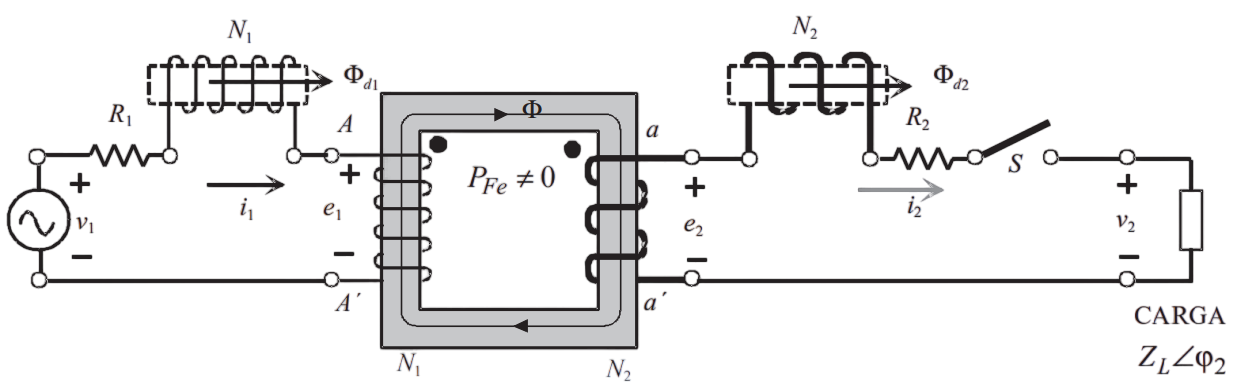
\includegraphics[width=0.8\linewidth]{trafo-real}
	\caption{Transformador real con bobinas ideales en el núcleo.}
	\label{fig:tranformador-real}
\end{figure} 

La aplicación del 2° Ley de Kirchhoff a los circuitos primario y secundario nos da:
\begin{equation*}
	\begin{split}
		v_1 = e_1 + R_1 i_1 + L_{d1} \dfrac{di_1}{dt}\\
		e_2 = v_2 + R_2 i_2 + L_{d2} \dfrac{di_2}{dt}
	\end{split}
\end{equation*}

Y expresado en forma fasorial, las tensiones $\fasor{V}_1$ y $\fasor{V}_2$ se pueden calcular como:
\begin{equation*}
	\begin{split}
		\fasor{v}_{1} = \fasor{e}_{1} + R_{1}  \fasor{i}_{1} + j X_{2} \fasor{i}_{2} \\
		\fasor{v}_{2} = \fasor{e}_{2} - R_{2} \fasor{i}_{2} - j X_{2} \fasor{i}_{2}
	\end{split}
\end{equation*}
 
Como se puede apreciar, las caídas de tensión $V_{1}$ y $V_{2}$ no son iguales a $E_{1}$ y $E_{2}$ por lo tanto la relación de transformación para trafos reales queda:
\begin{equation}
	\dfrac{E_{1}}{E_{2}}=\dfrac{N_{1}}{N_{2}}=m
	\label{eq:rel-transf-real}
\end{equation}
En los transformadores industriales las caídas de tensión provocadas por el cobre son muy pequeñas por lo que podemos decir que:
\begin{equation}
	V_{1} \approx E_{1} \hspace{5mm}  V_{2} \approx E_{2}  \hspace{5mm} \therefore \hspace{5mm} \dfrac{V_{1}}{V_{2}} \approx m
\end{equation}

Si el transformador trabaja \textbf{en vacío}, $I_{2}=0$ por lo tanto las ecuaciones quedan:
\begin{equation*}
	\fasor{v}_{1} = \fasor{e}_{1} + R_{1} \fasor{i}_{0} + j X_{1} \fasor{i}_{0}  \hspace{.3cm};\hspace{.3cm}	\fasor{v}_{2} = \fasor{e}_{2}
\end{equation*}

Las caídas de tensiones por pérdidas son muy pequeñas en vacío por lo tanto:
\begin{equation}
	V_{1}=E_{1} \hspace{5mm} ; \hspace{5mm} V_{20}=E_{2} \hspace{5mm} \therefore \hspace{5mm} m=\dfrac{V_{1}}{V_{20}}=\dfrac{E_{1}}{E_{2}}=\dfrac{N_{1}}{N_{2}}
\end{equation}


Este cociente con la tensión secundaria en vacío $V_0$ es el que incluye el fabricante en la placa características de la máquina. La ecuación \ref{eq:corriente1} es válida a todos los efectos.

\subsection{Circuito equivalente de un transformador}
Para el desarrollo de un circuito equivalente de un transformador se inicia \textbf{reduciendo} un devanado al mismo número de espiras que el otro. Si reducimos el secundario al primario, entonces $N_{1}=N'_{2}$. Para que este nuevo transformador sea equivalente al original \textsl{deben conservarse las potencias activa y reactiva}, y su distribución en los distintos elementos del circuito secundario. 
\begin{figure}[H]
	\centering
	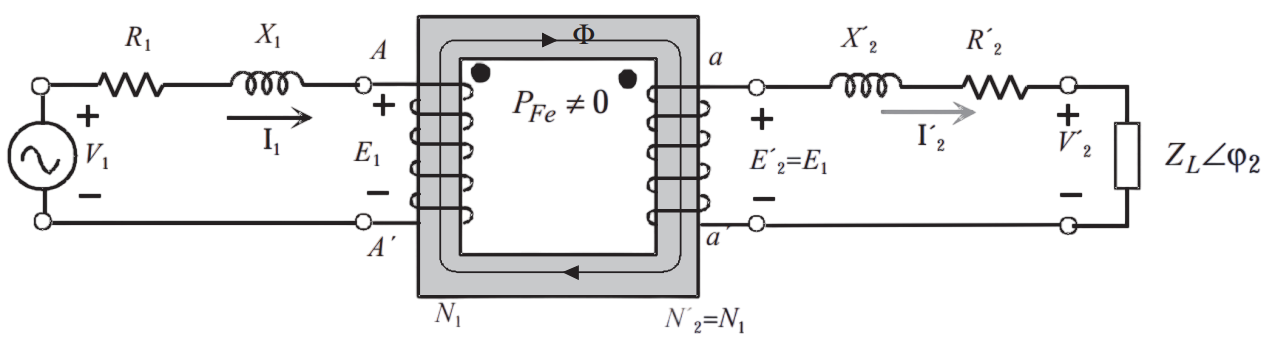
\includegraphics[width=0.8\linewidth]{trafo-equivalente}
	\caption{Circuito equivalente de un transformador real reducido al primario}
\end{figure} 

\begin{enumerate}[label=\textbf{\alph*)}]
	\item \textbf{F.m.m.s. y Tensiones}
	
	Si el número de espiras en el primer devanado y el segundo devanado reducido son iguales, y considerando la relación de transformación de la ecuación \ref{eq:rel-transf-real}, entonces se tiene que:
	\begin{equation*}
		\dfrac{E_1}{E_2'} = \dfrac{N_1}{N_2'} = 1
	\end{equation*}

	Entonces, las tensiones reducidas se calculan como sigue:
	\begin{equation}
			\begin{split}
				E_2' = m E_2 \\
				V_2' = m V_2
			\end{split}
		\label{eq:v-reducida}
	\end{equation}
	
	\item \textbf{Corrientes}
	
	
	Como la potencia aparente en ambos secundarios se conserva $S_{2}=V_{2}\, I_{2}=V'_{2}\, I'_{2}$ reemplazando $V'_{2}$ de la ecuación \ref{eq:v-reducida} queda:
	\begin{equation}
		I'_{2}=\dfrac{I_{2}}{m}
		\label{eq:i-reducida}
	\end{equation}


	\item \textbf{Impedancias}
	
	
	Como la potencia activa se conserva $P = R_{2}\, {I_{2}}^{2} = R'_{2} \, {I'_{2}}^{2}$ reemplazando $I'_{2}$ de la ecuación \ref{eq:i-reducida} se tiene que:
	\begin{equation}
		R'_{2}=m^{2}\, R_{2}
	\end{equation}
	Lo mismo sucede con la potencia reactiva por lo tanto:
	\begin{equation}
		X'_{2}=m^{2}\, X_{2}
	\end{equation}
	Entonces para una impedancia $Z'_{L}=m^{2}\, Z_{L}$.
\end{enumerate}

La importancia fundamental de la reducción de los devanados es obtener una representación del transformador donde no exista una relación de transformación porque los devanados son iguales, es decir, $N_{1}=N'_{2}$. Además, se pudo sustituir los devanados acoplados magnéticamente por otros \textbf{acoplados sólo eléctricamente}.\\


Teniendo en cuenta que los devanados idénticos tienen la misma polaridad, se puede sustituir a los mismos por un solo devanado como se muestra en la figura \ref{fig:trafo-un-devanado}. Por dicho devanado circulará una corriente $\fasor{i}_1 - \fasor{i}_2'$, lo cual, según las ecuaciones \ref{eq:corriente1} y \ref{eq:i-reducida}, $\fasor{i}_0$ circulará por el devanado.


\begin{figure}[H]
	\centering
	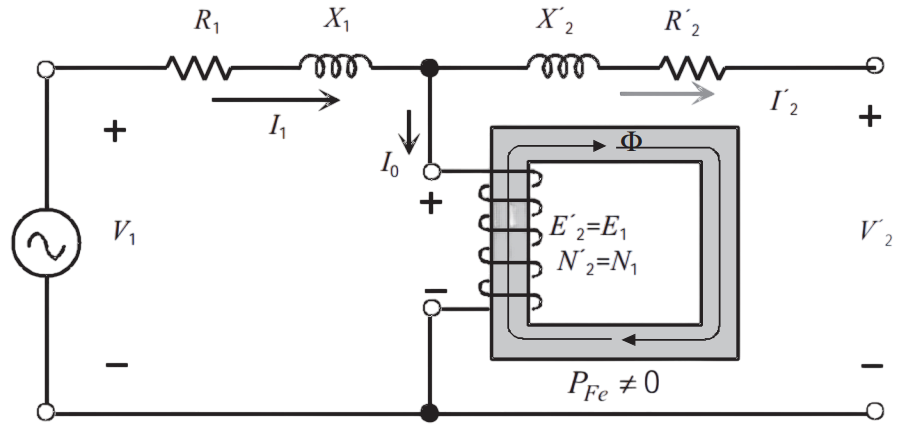
\includegraphics[width = .6\linewidth]{trafo-equivalente-2}
	\caption{Circuito equivalente de un transformador real reducido al primario.}
	\label{fig:trafo-un-devanado}
\end{figure}

%Acá falta agregar la referencia a la unidad 1, pero lo voy a hacer cuando esté la unidad xd
Según lo visto en la sección x de la Unidad 1, la corriente de vacío que circula por el devanado de $N_1=N_2'$ espiras, se puede descomponer en una parte activa $\fasor{i}_{Fe}$ y otra reactiva $\fasor{i}_\mu$, y se representa con un circuito en paralelo formado por una resistencia $R_{Fe}$, cuyas pérdidas por calor indican las \textsl{pérdidas en el hierro}; y por una reactancia $X_{\mu}$, por la que se deriva la corriente de magnetización de la máquina.\\


Conforme a lo mencionado, el circuito de la figura \ref{fig:circuito-equivalente-exacto} representa al \textbf{circuito equivalente exacto del transformador} reducido al primario.\\


\textsl{``Este circuito responde fielmente al comportamiento del transformador real y por ello se denomina circuito equivalente \textbf{exacto}.''} %\cite{ME_JFM}.

\begin{figure}[H]
	\centering
	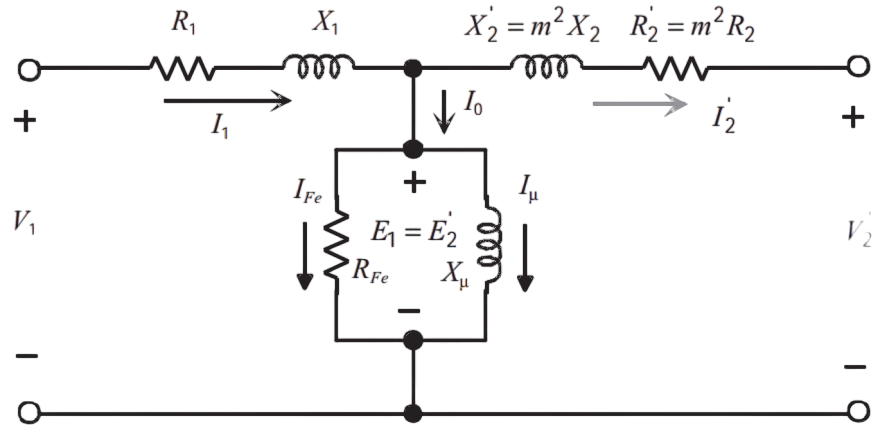
\includegraphics[width = .6 \linewidth]{circuito-equivalente-exacto}
	\caption{Circuito equivalente exacto de un transformador real reducido al primario.}
	\label{fig:circuito-equivalente-exacto}
\end{figure}


El esquema puede simplificarse aún más observando la conexión en serie constituida por las ramas primaria y secundaria (reducida), obteniendo una impedancia compuesta por una \textsl{resistencia de cortocircuito} $R_{cc}$ y una \textsl{reactancia de cortocircuito} $X_{cc}$:
% Tengo que ver mejor cómo alinear esto
\begin{equation}
	\begin{aligned}
		R_{cc} &= R_1 + R_2'\\
		X_{cc} &= X_1 + X_2'
	\end{aligned}
\end{equation}

Entonces, el circuito de la figura \ref{fig:circuito-equivalente-exacto} se convierte en el de la figura \ref{fig:aproximado-2}

\begin{figure}[H]
	\centering
	\begin{subfigure}[b]{0.4\textwidth}
		\centering
		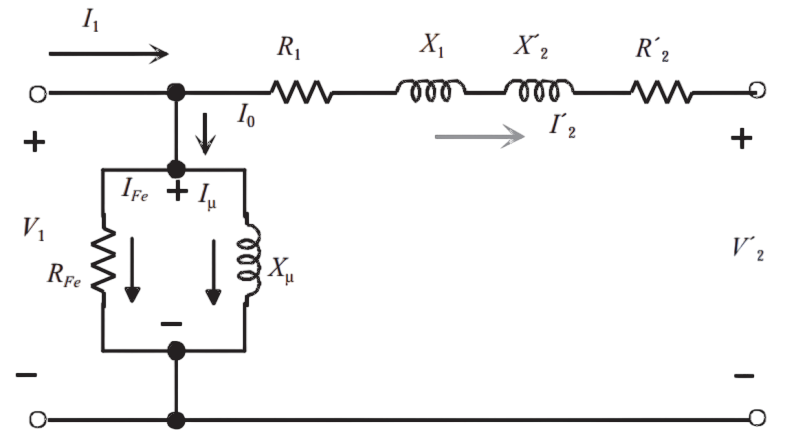
\includegraphics[height = 4cm]{equivalente-aproximado-1}
		\subcaption{}
		\label{fig:aproximado-1}
	\end{subfigure}
	\begin{subfigure}[b]{0.4\textwidth}
		\centering
		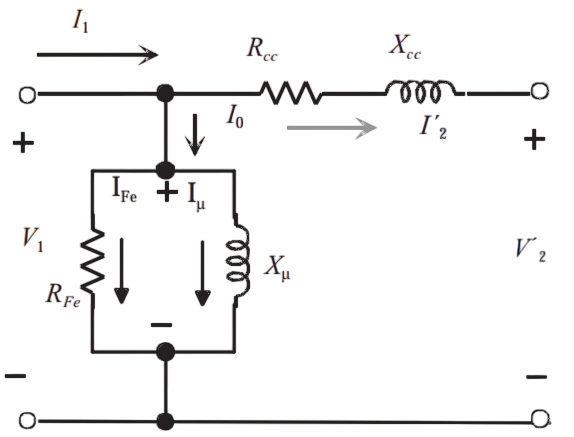
\includegraphics[height = 4cm]{equivalente-aproximado-2}
		\subcaption{}
		\label{fig:aproximado-2}
	\end{subfigure}
	\caption{Circuito equivalente aproximado de un transformador reducido al primario.}
\end{figure}

Con este último circuito equivalente simplificado se pueden resolver una variedad de problemas prácticos que afectan la utilización del transformador; en particular para el cálculo de la \textsl{caída de tensión} y el \textsl{rendimiento}. Inclusive, si solo se trata de la determinación de la caída de tensión del transformador, se puede despreciar la rama paralelo, ya que no afecta al cálculo.

\subsection{Ensayos del transformador}
